\documentclass[tikz,convert={density=150,size=600,outext=.png}]{standalone}
\usetikzlibrary{shapes, calc, arrows, fit, positioning, decorations, patterns, decorations.pathreplacing, chains, snakes}

\begin{document}
  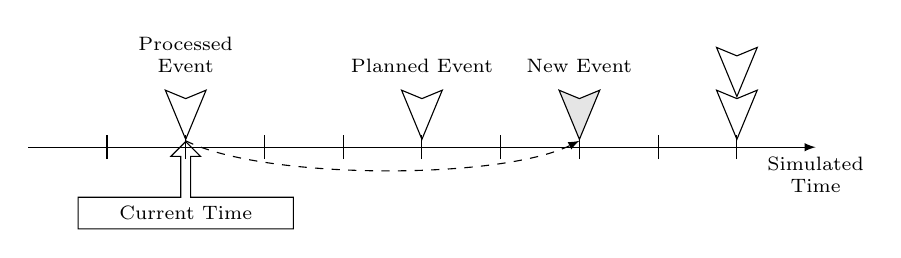
\begin{tikzpicture}[>=latex, font=\scriptsize]
    \draw[->] (0,0) -- (10,0) node[pos=1, below, align=center] (sim-time) {Simulated \\ Time};

    \foreach \x in { 1, 2, 3, 4, 5, 6, 7, 8, 9} {
        \draw (\x,-0.15) -- (\x,0.15) node (tick\x) {};
    };
    \node[shape=dart, draw, shape border rotate=270 ] at (2, 0.5) (currevent) {};
    \node[draw, arrow box, arrow box arrows={north:.7cm}, text width=2.5cm, align=center, below = 0cm of currevent] (tsim) {Current Time};
    \node[align=center, above=0.2cm of currevent, text width=2cm]  {Processed Event};

    \node[shape=dart, draw, shape border rotate=270 ] at (5, 0.5) (futureevent) {};
    \node[align=center, above=0.2cm of futureevent, text width=2cm] {Planned Event};

    \node[fill=black!10, shape=dart, draw, shape border rotate=270 ] at (7, 0.5) (newbornevent) {};
    \node[align=center, above=0.2cm of newbornevent, text width=1.5cm] {New Event};

    \node[shape=dart, draw, shape border rotate=270 ] at (9, 0.5) (futureevent2) {};
    \node[shape=dart, draw, shape border rotate=270, above=0cm of futureevent2 ] (futureevent3) {};

    \draw[dashed, ->] (currevent.south) .. controls +(1,-0.5) and +(-1,-0.5) .. (newbornevent.south);
  \end{tikzpicture}
\end{document}
